\section*{\centering\large{INFORME DE TAREA MÁS SIGNIFICATIVA}}

\textbf{Tarea: Motores de Videojuegos}\\ 

\textbf{Descripción del proceso:}\\ 

Un motor de videojuegos es un software específicamente para facilitar el desarrollo y la creación de videojuegos. Es una colección de herramientas, bibliotecas y sistemas que permiten a los desarrolladores de juegos crear, diseñar y programar juegos de manera mas eficiente.

El motor de un videojuego proporciona una serie de funcionalidades básicas que son necesarias para la creación de juegos, como la representación gráfica en 2D o 3D, la gestión del sonido, la física del juego, la inteligencia artificial, el manejo de colisiones, la animación, la gestión de recursos y otros aspectos técnicos. También suele incluir herramientas de desarrollo, como un editor de niveles, un sistema de scripting o un depurador, que ayudan a los desarrolladores a crear contenido y a depurar sus juegos.

Los motores de videojuegos permiten a los desarrolladores centrarse en la creación de contenido y la jugabilidad, en lugar de tener que preocuparse por programar desde cero todas las funcionalidades básicas de un juego. Al utilizar un motor de videojuegos, los desarrolladores pueden ahorrar tiempo y esfuerzo, ya que muchas tareas técnicas complejas están predefinidas y listas para usar.

Existen diferentes motores de videojuegos disponibles en la industria, como Unity, Unreal Engine, CryEngine y Godot, entre otros. Cada motor tiene sus propias características, fortalezas y limitaciones, y los desarrolladores pueden elegir el que mejor se adapte a sus necesidades y habilidades.

\textbf{VENTAJAS}

\begin{itemize}
	\item \textbf{Ahorro de tiempo:} proporcionan una base sólida y una serie de herramientas preconstruidas.
	
	\item \textbf{Flexibilidad:} permiten personalizar y ajustar los aspectos técnicos del juego según necesidades específicas.
	
	\item\textbf{Multiplataforma:} permiten crear juegos para distintas plataformas.
	
	\item\textbf{Comunidad:} tienen una gran comunidad de desarrolladores que comparten recursos, consejos y soluciones a problemas.
\end{itemize}
\newpage
\textbf{DESVENTAJAS}

\begin{itemize}
	\item \textbf{Costo:} algunos motores pueden ser bastante costoso, especialmente para pequeños estudios o independientes.
	
	\item \textbf{Limitaciones creativas:} pueden proporcionar una estructura base para el desarrollo del juego, pero también pueden limitar la creatividad y la libertad del desarrollador.
	
	\item \textbf{Curva de aprendizaje:} algunos motores pueden requerir conocimientos avanzados de programación y habilidades técnicas.
	
	\item \textbf{Dependencia del motor:} pueden hacer que el desarrollador sea dependiente de ese motor especifico por sus características.
\end{itemize}

\begin{figure}[!ht]
	\centering
	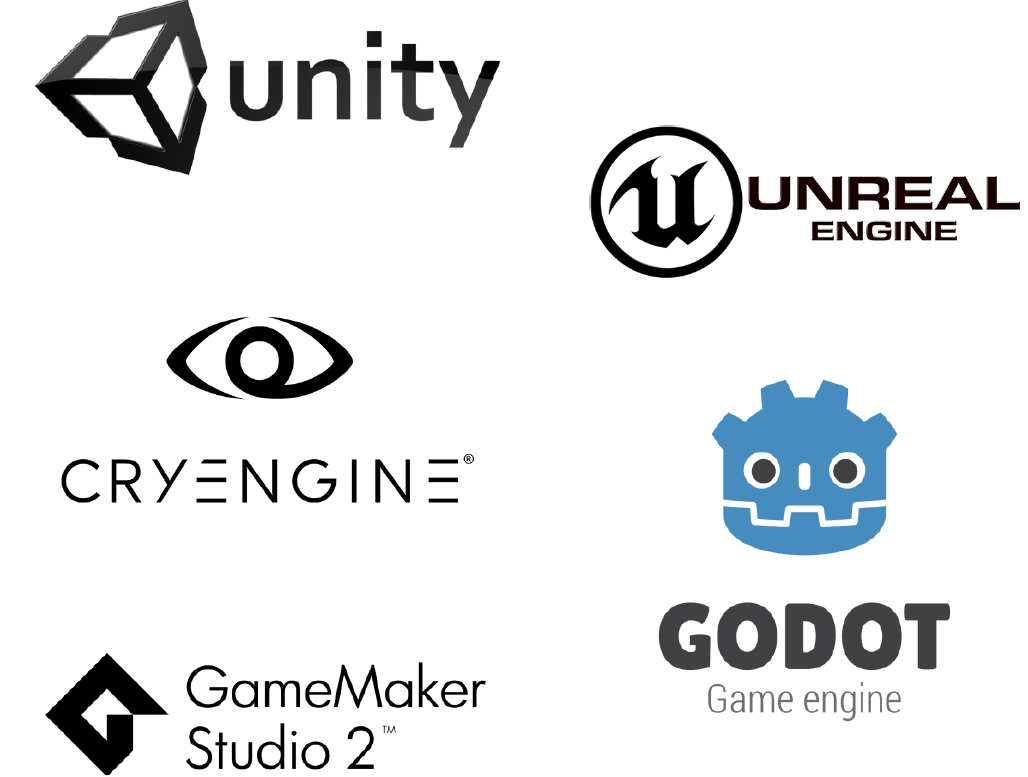
\includegraphics[scale=0.7]{Imágenes/motor.png}
\end{figure}
\newpage
\subsection{Importación de modelos a Unity}

Para importar un modelo a Unity, sigue los siguientes pasos:

\begin{enumerate}
	\item Preparación del modelo: Antes de importar el modelo a Unity, asegúrate de que el modelo esté en un formato compatible. Unity admite varios formatos de modelos 3D, como FBX, OBJ y Collada (DAE). Si tu modelo no está en uno de estos formatos, deberás convertirlo usando herramientas como Blender u otros software de modelado 3D.
	
	\item Creación de una carpeta de recursos: En el proyecto de Unity, crea una carpeta en la que puedas almacenar los recursos del modelo. Por ejemplo, puedes crear una carpeta llamada "Modelos".
	
	\item Importación del modelo: Arrastra y suelta el archivo del modelo en la carpeta de recursos que creaste. Unity comenzará a importar automáticamente el modelo y sus texturas asociadas si las hay. Puedes ver el progreso de la importación en la barra de progreso de Unity.
	
	\item Ajuste de las propiedades del modelo: Una vez que el modelo esté importado, puedes ajustar sus propiedades en el inspector de Unity. Esto incluye la escala, la posición, la rotación y otros ajustes específicos del modelo.
	
	\item Uso del modelo en la escena: Ahora puedes utilizar el modelo importado en tu escena. Arrastra y suelta el modelo desde la carpeta de recursos a la jerarquía de objetos de la escena o colócalo mediante scripts en tiempo de ejecución.
\end{enumerate}